\chapter{Phương pháp đề xuất}
\label{Chapter3}

\section{Phân loại zero-shot với BioMedCLIP và định hướng cải tiến}
\label{sec:ch3_biomedclip_baseline}

Với việc được tiền huấn luyện trên PMC-15M, một tập dữ liệu y sinh quy mô lớn có bao gồm ảnh X-quang, BioMedCLIP \cite{BiomedCLIP} được lựa chọn làm mô hình nền tảng để phát triển hệ thống phân loại. Trước khi xây dựng phương pháp đề xuất, nhóm khảo sát khả năng chuyển trực tiếp tri thức của mô hình sang bài toán phân loại ảnh X-quang xương trong thiết lập \textit{zero-shot}. Khảo sát này giúp làm rõ cơ chế phân loại ban đầu của BioMedCLIP và xác định những khía cạnh cần thích nghi với dữ liệu đích.

Phần này tập trung mô tả quy trình phân loại và các định hướng cải tiến. Thiết kế thực nghiệm được trình bày tại Mục \ref{sec:experiment_content}, còn kết quả định lượng và phần bàn luận tương ứng được trình bày tại Mục \ref{subsec:foundation_model_evaluation} của Chương 4 để tránh lặp lại nội dung thực nghiệm trong chương phương pháp.

\subsection{Quá trình phân loại của BioMedCLIP}
\label{subsec:ch3_biomedclip_classification}

BioMedCLIP trong thiết lập \textit{zero-shot} thực hiện phân loại dựa trên cơ chế đối sánh ảnh-văn bản thay vì sử dụng một đầu phân loại được huấn luyện trên dữ liệu đích. Quy trình gồm năm bước chính:

\begin{enumerate}
    \item \textbf{Xây dựng câu nhắc văn bản:} Với mỗi lớp, tên bệnh lý được đưa vào một câu nhắc mô tả ảnh X-quang, chẳng hạn \texttt{A radiograph showing osteosarcoma.} đối với lớp sarcoma xương. Cùng một mẫu câu được áp dụng nhất quán cho toàn bộ tập lớp.
    \item \textbf{Trích xuất đặc trưng văn bản:} Câu nhắc của từng lớp được đưa qua nhánh mã hóa văn bản sử dụng kiến trúc PubMedBERT để tạo các vectơ đặc trưng lớp trong không gian biểu diễn chung.
    \item \textbf{Trích xuất đặc trưng hình ảnh:} Ảnh X-quang đầu vào được xử lý qua nhánh mã hóa thị giác sử dụng kiến trúc Vision Transformer để tạo vectơ đặc trưng đại diện cho thông tin thị giác.
    \item \textbf{Tính độ tương đồng:} Độ tương đồng côsin được tính giữa vectơ ảnh và vectơ văn bản của từng lớp. Cặp ảnh - văn bản có sự tương hợp cao nhất về mặt ngữ nghĩa y khoa sẽ đạt điểm số lớn nhất.
    \item \textbf{Đưa ra dự đoán:} Các điểm số tương đồng được chuẩn hóa thông qua hàm Softmax để chuyển thành phân phối xác suất. Lớp tương ứng với câu mô tả có xác suất cao nhất sẽ được lựa chọn làm kết quả dự đoán của mô hình.
\end{enumerate}

\subsection{Định hướng cải tiến}
\label{subsec:ch3_improvement_directions}

Các kết quả và phân tích ở Chương 4 cho thấy mô hình nền tảng có khả năng phân biệt ban đầu nhưng chưa thể áp dụng trực tiếp cho bài toán đích. Từ những hạn chế đó, nghiên cứu đề xuất các cải tiến sau:

\textbf{Tinh chỉnh với dữ liệu hạn chế:} LoRA được lựa chọn vì đây là phương pháp tinh chỉnh hiệu quả về tham số, cho phép thích nghi BioMedCLIP với miền ảnh X-quang xương mà vẫn bảo toàn phần lớn tri thức tiền huấn luyện. So với tinh chỉnh toàn bộ tham số, LoRA giúp giảm số tham số cần cập nhật và hạn chế nguy cơ quá khớp trong bối cảnh dữ liệu y khoa có quy mô hạn chế, phân bố lớp không đồng đều. Mặc dù nghiên cứu sử dụng toàn bộ dữ liệu hiện có trong thiết lập chính, nhiều lớp vẫn chỉ chứa số lượng mẫu nhỏ; vì vậy, phương pháp cũng được đánh giá trong các kịch bản học ít mẫu.

\textbf{Bảo toàn thông tin ảnh cục bộ:} Việc co toàn bộ ảnh X-quang độ phân giải cao về kích thước đầu vào cố định có thể làm mất các chi tiết tổn thương nhỏ. Nhánh ảnh vì vậy kết hợp ảnh toàn cục với các vùng cục bộ giàu thông tin (global-local), đồng thời bổ sung biểu diễn vị trí để duy trì cả bối cảnh giải phẫu và bằng chứng hình thái tại chỗ.

\textbf{Lựa chọn mục tiêu huấn luyện biểu diễn:} Hàm mất mát tương phản gốc InfoNCE xem các cặp khác mẫu trong cùng lô là âm, kể cả khi chúng thuộc cùng một lớp và có nội dung lâm sàng liên quan. Nghiên cứu sử dụng hàm mất mát khớp ngữ nghĩa (Semantic Matching Loss) với phân phối đích mềm theo nhãn lớp, nhờ đó vẫn ưu tiên cặp ảnh - văn bản đúng của từng mẫu nhưng giảm ảnh hưởng của các cặp âm tính giả giữa những mẫu cùng lớp.

\textbf{Khai thác thông tin lâm sàng:} Thiết lập zero-shot chỉ đối sánh ảnh với câu nhắc lớp và không sử dụng bệnh sử riêng của người bệnh. Phương pháp đề xuất bổ sung nhánh văn bản để mã hóa thông tin lâm sàng, sau đó sử dụng chú ý chéo hai chiều nhằm học quan hệ giữa dấu hiệu trên ảnh với ngữ cảnh bệnh sử. Chẩn đoán xác định và nhãn phân loại không được nối trực tiếp vào văn bản đầu vào; những giới hạn còn lại của nguồn văn bản thực tế được trình bày cùng quá trình chuẩn bị dữ liệu ở Chương 4.

\textbf{Xử lý phân loại đa lớp và mất cân bằng dữ liệu:} Hai bộ dữ liệu được thiết lập dưới dạng phân loại đơn nhãn đa lớp với phân bố lớp mất cân bằng. XBone-Net sử dụng mạng nguyên mẫu với tâm lớp thực nghiệm để đưa ra quyết định theo khoảng cách trong không gian biểu diễn, kết hợp entropy chéo có trọng số dựa trên số lượng mẫu hiệu dụng để hạn chế mất cân bằng lớp. Không gian biểu diễn xây dựng bởi mạng nguyên mẫu tạo cơ sở cho cơ cơ chế phát hiện dữ liệu ngoài phân phối dựa trên khoảng cách.

\textbf{Phát hiện dữ liệu ngoài phân phối:} Ngoài dự đoán lớp, nghiên cứu bổ sung mô-đun hậu xử lý OOD dựa trên hình học của không gian biểu diễn đã học. Mô-đun này không thay đổi quá trình huấn luyện bộ phân loại và không yêu cầu mẫu OOD để cập nhật tham số. Các điểm bất thường được phát hiện dựa trên khoảng cách đến tâm lớp, trong đó khoảng cách Mahalanobis được sử dụng trong mô tả suy luận chính, cùng các phương án hậu xử lý đối chứng được đánh giá riêng ở Chương 4.

Các định hướng trên được hiện thực hóa trong XBone-Net và được trình bày chi tiết ở các phần tiếp theo.

\section{Tổng quan phương pháp đề xuất}
\label{sec:final-pipeline}

Nhóm nghiên cứu đề xuất XBone-Net cho bài toán phân loại đa lớp ảnh X-quang xương có kết hợp thông tin lâm sàng. Hệ thống được xây dựng theo kiến trúc hai nhánh. Nhánh ảnh khai thác đồng thời cấu trúc giải phẫu toàn cục và các vùng cục bộ giàu chi tiết, trong khi nhánh văn bản biểu diễn bệnh sử và lý do vào viện. Hai nguồn thông tin được ánh xạ vào cùng một không gian đặc trưng, trao đổi ngữ cảnh bằng cơ chế chú ý chéo hai chiều, sau đó được phân loại bằng mạng nguyên mẫu.

\begin{figure}[H]
    \centering
    
\includegraphics[width=\textwidth]{images/tongquat.png}
    \caption{Sơ đồ tổng quan phương pháp XBone-Net đề xuất}
    \label{fig:ch3_overview}
\end{figure}

Như minh họa trong Hình \ref{fig:ch3_overview}, XBone-Net kế thừa bộ mã hóa thị giác và bộ mã hóa văn bản của BiomedCLIP \cite{BiomedCLIP}. Các tham số nền được giữ cố định để bảo toàn tri thức y sinh đã học trước, trong khi các ma trận thích nghi hạng thấp LoRA \cite{Hu2022LoRA} được huấn luyện trên dữ liệu đích. Sau bước mã hóa, mô-đun dung hợp kết hợp đặc trưng toàn cục và cục bộ của hai phương thức. Biểu diễn tổng hợp cuối cùng được so sánh với các nguyên mẫu lớp để đưa ra dự đoán.

Mỗi mẫu dữ liệu được ký hiệu bởi bộ ba gồm ảnh X-quang, thông tin lâm sàng và nhãn lớp. Tập huấn luyện có dạng:

\begin{equation}
\mathcal{D}_{\mathrm{train}}
=
\left\{
\left(x_i^{img},x_i^{txt},y_i\right)
\right\}_{i=1}^{N},
\qquad
y_i\in\mathcal{Y}.
\label{eq:ch3_dataset}
\end{equation}

Trong Công thức \ref{eq:ch3_dataset}, $x_i^{img}$ là ảnh X-quang của mẫu thứ $i$, với $x_i^{img}\in\mathrm{R}^{H\times W\times C}$, trong đó $H$, $W$ và $C$ lần lượt là chiều cao, chiều rộng và số kênh của ảnh. Thông tin lâm sàng được ký hiệu $x_i^{txt}=\left(w_{i,1},\ldots,w_{i,T_i}\right)$, trong đó $T_i$ là số đơn vị mã hóa. Nhãn $y_i$ thuộc tập lớp $\mathcal{Y}=\left\{y_1,y_2,\ldots,y_K\right\}$; và $N$ là số mẫu huấn luyện. Thông tin lâm sàng được sử dụng làm đầu vào không bao gồm kết luận chẩn đoán rút ra trực tiếp từ ảnh X-quang. Quy ước này giúp hạn chế hiện tượng mô hình dựa vào từ khóa chẩn đoán thay vì học mối liên hệ giữa biểu hiện hình ảnh và bệnh cảnh.

Quá trình xây dựng mô hình được chia thành hai giai đoạn ngoại tuyến. Giai đoạn thứ nhất thích nghi hai nhánh mã hóa và căn chỉnh không gian ảnh-văn bản bằng hàm mất mát khớp ngữ nghĩa. Giai đoạn thứ hai học cơ chế dung hợp và ranh giới phân loại trong không gian nguyên mẫu. Khi suy luận trực tuyến, toàn bộ tham số và các nguyên mẫu lớp được cố định, mô hình chỉ thực hiện tính toán truyền thuận cho một ca mới.

\section{Nhánh biểu diễn ảnh}
\label{sec:ch3_image_branch}

\subsection{Tiền xử lý ảnh X-quang và xử lý độ phân giải cao}
\label{subsec:ch3_image_preprocessing}
\label{subsec:ch3_high_resolution}

Ảnh X-quang đầu vào $x_i^{img}$ có kích thước và tỷ lệ khung hình khác nhau, trong khi bộ mã hóa thị giác của BioMedCLIP nhận ảnh vuông $224\times224$. Để giữ đồng thời bố cục chung và chi tiết cục bộ, mỗi ảnh được chuyển thành một ảnh toàn cục $x_i^{img,g}$ và bốn ảnh cục bộ $\{x_{i,m}^{img,\ell}\}_{m=1}^{4}$. Việc chọn vùng chỉ sử dụng giá trị điểm ảnh, không sử dụng nhãn, bệnh sử hoặc chú thích tổn thương.

\begin{figure}[H]
    \centering
    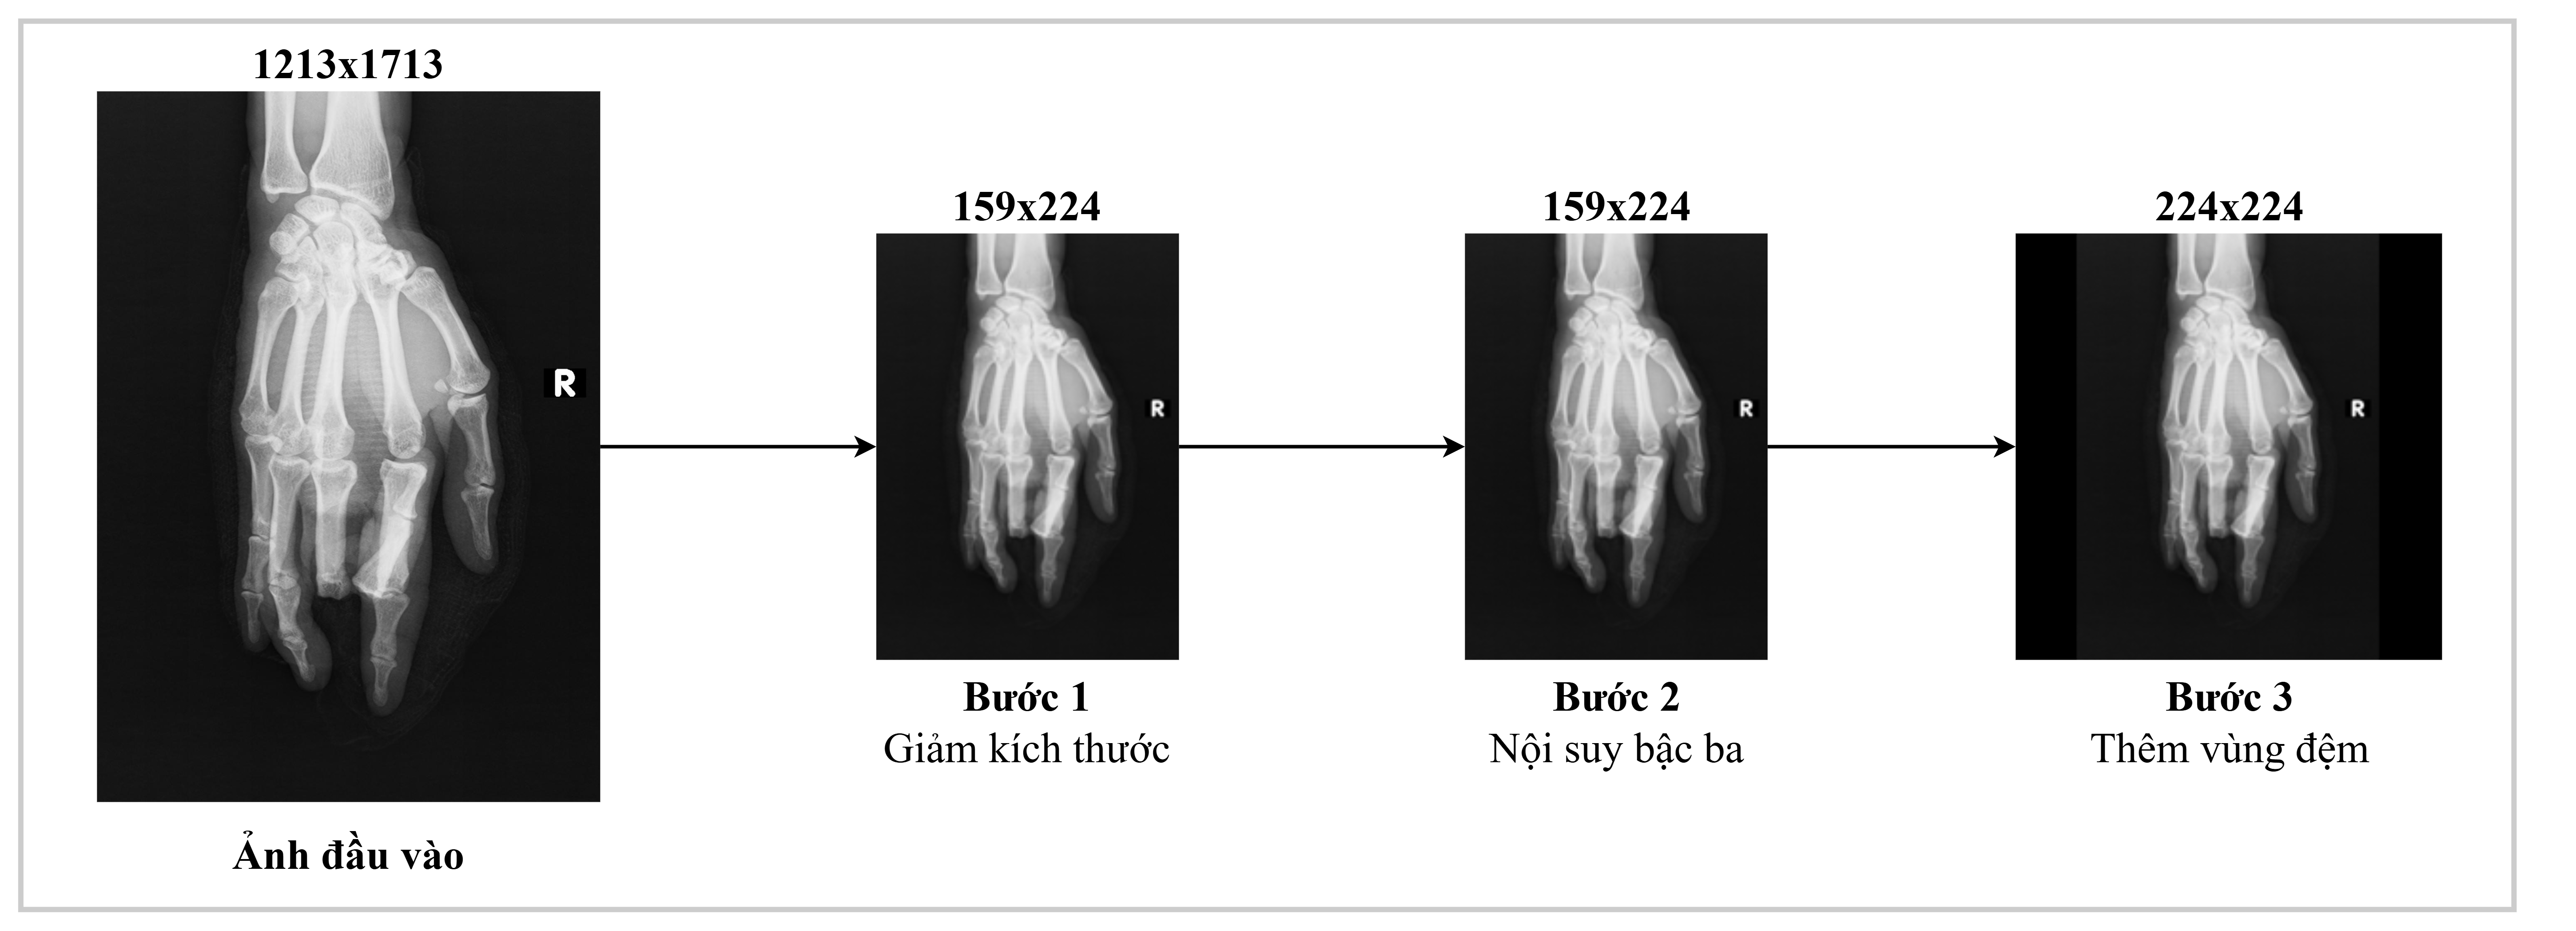
\includegraphics[width=\textwidth]{images/ImagePreprocess.png}
    \caption{Quy trình tạo ảnh toàn cục và bốn ảnh cục bộ từ ảnh X-quang}
    \label{fig:ch3_high_resolution_preprocessing}
\end{figure}

\subsubsection{Xác định vùng nội dung và tạo ảnh toàn cục}

Ảnh được chuyển sang thang xám và chuẩn hóa cường độ về $[0,1]$. Trên phiên bản có cạnh dài không quá $512$ điểm ảnh, mức nền được ước lượng bằng trung vị của dải biên. Mặt nạ tiền cảnh được xác định bởi:

\begin{equation}
\begin{aligned}
\mu_i^{\partial}
&=\operatorname{median}_{p\in\partial x_i}x_i^{gray}(p),\\
\sigma_i^{\partial}
&=1{,}4826\operatorname{median}_{p\in\partial x_i}
\left|x_i^{gray}(p)-\mu_i^{\partial}\right|,\\
m_i^{fg}(p)
&=\mathbb{I}\!\left(
\left|x_i^{gray}(p)-\mu_i^{\partial}\right|
\geq\max\!\left(0{,}035,4\sigma_i^{\partial}\right)
\right).
\end{aligned}
\label{eq:ch3_foreground_mask}
\end{equation}

Ở đây, $p$ là vị trí điểm ảnh, $\partial x_i$ là dải biên, $\mu_i^{\partial}$ và $\sigma_i^{\partial}$ lần lượt là mức nền và độ phân tán bền vững tại biên, còn $\mathbb{I}(\cdot)$ là hàm chỉ thị. Các hàng và cột có ít nhất $1\%$ điểm ảnh tiền cảnh được dùng để xác định hộp nội dung và các đoạn liên tục ngắn hơn $3\%$ chiều tương ứng bị loại và hộp được mở rộng thêm $4\%$. Nếu chiều rộng hoặc chiều cao của hộp dưới $35\%$ kích thước ảnh, diện tích dưới $20\%$ hoặc năng lượng tương phản được giữ lại dưới $95\%$, quy trình sử dụng toàn bộ ảnh để hạn chế cắt mất cấu trúc giải phẫu.

Vùng nội dung được đổi kích thước đồng nhất trên hai trục bằng nội suy hai chiều bậc ba, sau đó đệm thành ảnh vuông $224\times224$. Màu đệm là trung vị màu của dải biên thay vì một giá trị cố định:

\begin{equation}
x_i^{img,g}
=\mathcal{T}_{I}\!\left(
\mathcal{L}_{224}\!\left(
\mathcal{C}\!\left(x_i^{img};m_i^{fg}\right)
\right)
\right).
\label{eq:ch3_global_image}
\end{equation}

$\mathcal{C}$ là phép cắt vùng nội dung, $\mathcal{L}_{224}$ là phép giữ tỷ lệ và đệm ảnh, còn $\mathcal{T}_{I}$ là phép chuẩn hóa đầu vào do BioMedCLIP cung cấp.

\subsubsection{Sinh và lựa chọn vùng cục bộ}

Vùng nội dung được thu nhỏ sao cho cạnh dài không vượt quá $896$ điểm ảnh và không phóng lớn ảnh nhỏ. Trên ảnh trung gian, quy trình sinh lưới cửa sổ $224\times224$ với bước dịch chuyển $168$ điểm ảnh ở vị trí cuối mỗi trục luôn được bổ sung để phủ phần biên. Gọi $\mathcal{G}_i$ là tập cửa sổ và $r_i(b)$ là tỷ lệ tiền cảnh trong cửa sổ $b$:

\begin{equation}
r_i(b)=\frac{1}{|b|}\sum_{p\in b}m_i^{fg}(p),
\qquad
\mathcal{B}_i=\{b\in\mathcal{G}_i\mid r_i(b)\geq0{,}60\}.
\label{eq:ch3_candidate_regions}
\end{equation}

Mặt nạ ở bước này được tính lại với mức nền là khoảng cường độ xuất hiện nhiều nhất tại biên. Mỗi cửa sổ được chấm điểm bằng mức biến thiên cục bộ, entropy mức xám và tỷ lệ tiền cảnh. Đáp ứng Laplacian làm nổi bật thay đổi cường độ \cite{Marr1980EdgeDetection} và thường được dùng để đo lượng chi tiết ảnh \cite{Pertuz2013FocusMeasures} còn entropy mô tả độ đa dạng của phân bố mức xám \cite{Shannon1948Information}:

\begin{equation}
\begin{aligned}
E_i(b)
&=\frac{1}{|b|}\sum_{(u,v)\in b}
\left|4x_i^{gray}(u,v)-\!\sum_{(u',v')\in\mathcal{N}_4(u,v)}
x_i^{gray}(u',v')\right|,\\
H_i(b)
&=-\frac{1}{\log_2 32}
\sum_{k:\,\pi_{i,k}(b)>0}\pi_{i,k}(b)\log_2\pi_{i,k}(b),\\
q_i(b)
&=0{,}55\widehat{E}_i(b)+0{,}35\widehat{H}_i(b)+0{,}10r_i(b).
\end{aligned}
\label{eq:ch3_candidate_score}
\end{equation}

$\mathcal{N}_4(u,v)$ là bốn điểm ảnh lân cận, $\pi_{i,k}(b)$ là tỷ lệ điểm ảnh thuộc khoảng mức xám thứ $k$, còn $\widehat{E}_i$ và $\widehat{H}_i$ là các giá trị được chuẩn hóa min--max trên $\mathcal{G}_i$; nếu mọi giá trị bằng nhau thì kết quả chuẩn hóa bằng $0$.

Bốn cửa sổ được chọn theo hai vai trò. Hai cửa sổ bao phủ nằm gần các vị trí phân bố đều trên trục dài của vùng nội dung. Hai cửa sổ tiêu điểm có điểm $q_i$ cao nhưng được khuyến khích cách xa các vùng đã chọn:

\begin{equation}
\begin{aligned}
b_{i,j}^{cov}
&=\underset{b\in\mathcal{B}_i\setminus\mathcal{S}_{i,j}}
{\operatorname{arg\,min}}
\frac{\|\boldsymbol{c}_i(b)-\boldsymbol{t}_{i,j}\|_2}
{0{,}5+0{,}5r_i(b)},\\
b_{i,j}^{foc}
&=\underset{b\in\mathcal{A}_{i,j}}
{\operatorname{arg\,max}}
\left[q_i(b)+0{,}35
\min_{a\in\mathcal{S}_{i,j}}
\|\boldsymbol{c}_i(b)-\boldsymbol{c}_i(a)\|_2\right].
\end{aligned}
\label{eq:ch3_region_selection}
\end{equation}

$\boldsymbol{c}_i(b)$ là tâm cửa sổ đã chuẩn hóa, $\boldsymbol{t}_{i,j}$ là vị trí bao phủ mục tiêu, $\mathcal{S}_{i,j}$ là các vùng đã chọn và $\mathcal{A}_{i,j}$ chỉ gồm các cửa sổ có mức giao trên hợp không quá $0{,}30$ với $\mathcal{S}_{i,j}$. Nếu có dưới bốn cửa sổ đạt ngưỡng tiền cảnh, toàn bộ lưới được xem xét. Nếu vẫn thiếu, quy trình lần lượt bỏ ràng buộc giao nhau và lặp vùng theo thứ tự xác định; nhờ đó mỗi ảnh luôn có đúng bốn đầu vào cục bộ.

Các cửa sổ được ánh xạ ngược về ảnh gốc trước khi cắt để tránh lấy chi tiết từ ảnh trung gian đã thu nhỏ. Mỗi vùng sau đó được giữ tỷ lệ, đệm và chuẩn hóa giống ảnh toàn cục:

\begin{equation}
x_{i,m}^{img,\ell}
=\mathcal{T}_{I}\!\left(
\mathcal{L}_{224}\!\left(x_i^{img}\!\mid_{b_{i,m}}\right)
\right),
\qquad m=1,\ldots,4.
\label{eq:ch3_local_images}
\end{equation}

Đầu ra tiền xử lý được viết gọn thành:

\begin{equation}
\left(
x_i^{img,g},
\{x_{i,m}^{img,\ell}\}_{m=1}^{4},
\{\boldsymbol{b}_{i,m}\}_{m=1}^{4}
\right),
\qquad
\boldsymbol{b}_{i,m}\in[0,1]^4.
\label{eq:ch3_preprocessing_output}
\end{equation}

$\boldsymbol{b}_{i,m}=(x_1,y_1,x_2,y_2)$ là hộp của vùng thứ $m$, được chuẩn hóa theo chiều rộng và chiều cao của ảnh gốc.

\subsection{Bộ mã hóa thị giác BioMedCLIP}
\label{subsec:ch3_visual_encoder}

Mô hình kế thừa bộ mã hóa của BioMedCLIP \cite{BiomedCLIP}, được xây dựng theo kiến trúc Vision Transformer \cite{Dosovitskiy2021ViT}. Mỗi ảnh $224\times224$ được chia thành lưới $14\times14$ mảnh ảnh kích thước $16\times16$. Sau khi thêm một đơn vị đại diện, bộ mã hóa và lớp chiếu tạo chuỗi gồm $197$ vectơ có chiều $D=512$:

\begin{equation}
\boldsymbol{H}_{i,m}^{I}
=\mathcal{F}_{I}\!\left(x_{i,m}\right)
=\left[
\boldsymbol{h}_{i,m,0};
\boldsymbol{h}_{i,m,1};\ldots;
\boldsymbol{h}_{i,m,196}
\right]
\in\mathbb{R}^{197\times D}.
\label{eq:ch3_visual_encoder}
\end{equation}

$\mathcal{F}_{I}$ gồm bộ mã hóa thị giác và lớp chiếu của BioMedCLIP. Chỉ số $m=g$ biểu thị ảnh toàn cục, còn $m=1,\ldots,4$ biểu thị bốn ảnh cục bộ. Chỉ số $0$ chỉ đơn vị đại diện, còn các chỉ số $1$ đến $196$ tương ứng với lưới mảnh ảnh. Ảnh toàn cục được biểu diễn bằng vectơ đại diện đã chuẩn hóa:

\begin{equation}
\boldsymbol{g}_i
=\operatorname{Norm}\!\left(\boldsymbol{h}_{i,g,0}\right)
\in\mathbb{R}^{D}.
\label{eq:ch3_global_visual_embedding}
\end{equation}

Ảnh toàn cục và bốn ảnh cục bộ dùng chung $\mathcal{F}_{I}$, do đó không hình thành một bộ mã hóa riêng cho nhánh cục bộ. Đối với mỗi ảnh cục bộ, lưới $14\times14$ được gộp trung bình thích nghi thành lưới $2\times2$; đơn vị đại diện của vùng được giữ lại. Vì vậy, mỗi vùng tạo năm đơn vị biểu diễn:

\begin{equation}
\boldsymbol{L}_{i,m}
=\operatorname{Norm}\!\left(
\left[
\boldsymbol{h}_{i,m,0};
\operatorname{Pool}_{2\times2}\!\left(
\boldsymbol{h}_{i,m,1:196}
\right)
\right]
\right)
\in\mathbb{R}^{5\times D}.
\label{eq:ch3_local_encoding}
\end{equation}

Phép $\operatorname{Norm}$ chuẩn hóa từng vectơ theo chuẩn $\ell_2$. Ghép kết quả của bốn vùng thu được $P=4\times5=20$ đơn vị cục bộ. Hộp của đơn vị đại diện bằng hộp của toàn vùng; bốn đơn vị còn lại nhận tọa độ của bốn ô con trong lưới $2\times2$.

Gọi $\boldsymbol{\ell}_{i,n}$ và $\boldsymbol{b}_{i,n}\in[0,1]^4$ lần lượt là đơn vị cục bộ thứ $n$ và hộp tọa độ tương ứng. Tọa độ được chiếu qua một mạng hai lớp, cộng có kiểm soát vào nội dung và chuẩn hóa lại:

\begin{equation}
\widetilde{\boldsymbol{\ell}}_{i,n}
=\operatorname{Norm}\!\left(
\operatorname{Norm}\!\left(\boldsymbol{\ell}_{i,n}\right)
+\tanh(\gamma)\,
\operatorname{Norm}\!\left(\mathcal{P}_{s}(\boldsymbol{b}_{i,n})\right)
\right),
\qquad n=1,\ldots,P.
\label{eq:ch3_spatial_encoding}
\end{equation}

$\mathcal{P}_{s}:\mathbb{R}^{4}\rightarrow\mathbb{R}^{D}$ là phép chiếu tọa độ và $\gamma$ là hệ số học được, khởi tạo bằng $0{,}1$. Cấu hình chính truyền nguyên 20 đơn vị sau khi bổ sung tọa độ, không gộp chúng bằng các truy vấn học được. Chuỗi thị giác dùng cho dung hợp vì vậy là:

\begin{equation}
\boldsymbol{V}_{i}
=\left[
\boldsymbol{g}_{i};
\widetilde{\boldsymbol{\ell}}_{i,1};\ldots;
\widetilde{\boldsymbol{\ell}}_{i,20}
\right]
\in\mathbb{R}^{21\times512}.
\label{eq:ch3_visual_sequence}
\end{equation}

Trong giai đoạn khớp ngữ nghĩa, chuỗi này được rút thành một vectơ ảnh. Trọng số của mỗi đơn vị cục bộ được điều kiện hóa bởi đặc trưng toàn cục, sau đó tóm tắt cục bộ được cộng vào đặc trưng toàn cục với hệ số $0{,}25$:

\begin{equation}
\begin{aligned}
e_{i,n}
&=\boldsymbol{w}^{\mathsf T}
\tanh\!\left(
\boldsymbol{W}_{\ell}\widetilde{\boldsymbol{\ell}}_{i,n}
+\boldsymbol{W}_{g}\boldsymbol{g}_i
\right),
\qquad
\alpha_{i,n}=\frac{\exp(e_{i,n})}{\sum_{r=1}^{P}\exp(e_{i,r})},\\
\overline{\boldsymbol{v}}_i
&=\operatorname{Norm}\!\left(
\boldsymbol{g}_i+0{,}25\operatorname{Norm}\!\left(
\sum_{n=1}^{P}\alpha_{i,n}
\widetilde{\boldsymbol{\ell}}_{i,n}
\right)
\right).
\end{aligned}
\label{eq:ch3_phase1_visual_summary}
\end{equation}

$\boldsymbol{W}_{\ell}$, $\boldsymbol{W}_{g}$ và $\boldsymbol{w}$ là các tham số của phép gộp có trọng số. Lớp tính điểm được khởi tạo bằng $0$, nên phép gộp ban đầu tương đương trung bình đều và chỉ thay đổi khi được huấn luyện. Ở giai đoạn dung hợp, mô hình sử dụng trực tiếp chuỗi $\boldsymbol{V}_i$ thay cho vectơ tóm tắt.

\section{Nhánh biểu diễn văn bản}
\label{sec:ch3_text_branch}

\subsection{Tiền xử lý thông tin lâm sàng}
\label{subsec:ch3_text_preprocessing}

Thông tin lâm sàng được chuẩn hóa về mã ký tự, khoảng trắng và dấu câu. Các trường thiếu hoặc ký hiệu không mang nội dung được xử lý thống nhất trước khi tách thành các đơn vị mã hóa. Chuỗi đầu vào được cắt hoặc đệm đến độ dài cho phép, đồng thời tạo mặt nạ để phân biệt nội dung thật với phần đệm:

\begin{equation}
\left(
\boldsymbol{u}_{i},
\boldsymbol{m}_{i}
\right)
=
\mathcal{T}_{T}\left(x_i^{txt}\right),
\label{eq:ch3_text_preprocessing}
\end{equation}

trong đó $\boldsymbol{u}_{i}$ là chuỗi chỉ số đơn vị mã hóa, $\boldsymbol{m}_{i}$ là mặt nạ chú ý và $\mathcal{T}_{T}$ là phép tiền xử lý văn bản.

\subsection{Bộ mã hóa văn bản}
\label{subsec:ch3_text_encoder}

Bộ mã hóa văn bản được kế thừa từ nhánh PubMedBERT của BiomedCLIP. Thành phần này tiếp nhận chuỗi đã mã hóa và tạo đặc trưng theo từng vị trí:

\begin{equation}
\boldsymbol{H}_{i}^{T}
=
\mathcal{P}_{T}
\left(
\mathcal{E}_{T}
\left(
\boldsymbol{u}_{i},
\boldsymbol{m}_{i}
\right)
\right)
\in
\mathbb{R}^{T_T\times D}.
\label{eq:ch3_text_encoder}
\end{equation}

Trong Công thức \ref{eq:ch3_text_encoder}, $\mathcal{E}_{T}$ là bộ mã hóa văn bản, $\mathcal{P}_{T}$ là phép chiếu sang không gian chung, $T_T$ là độ dài chuỗi và $D$ là số chiều đặc trưng. Phần tử đại diện đầu chuỗi được dùng làm đặc trưng văn bản toàn cục:

\begin{equation}
\boldsymbol{t}_{i}
=
\operatorname{Norm}_{2}
\left(
\boldsymbol{H}_{i,0}^{T}
\right).
\label{eq:ch3_global_text}
\end{equation}

Các phần tử còn lại của $\boldsymbol{H}_{i}^{T}$ được giữ lại để cơ chế chú ý chéo có thể liên hệ từng khái niệm lâm sàng với bằng chứng ảnh. Tương tự nhánh thị giác, khóa luận chỉ mô tả đầu vào và đầu ra cần thiết của bộ mã hóa, không phân tích sâu từng lớp Transformer đã được trình bày trong kiến trúc BiomedCLIP.

\section{Thích nghi tham số bằng LoRA}
\label{sec:ch3_lora}

Hai bộ mã hóa đã được tiền huấn luyện trên dữ liệu y sinh quy mô lớn, nhưng dữ liệu X-quang xương đích vẫn có khác biệt về phân bố ảnh, cách ghi bệnh sử và hệ thống nhãn. Việc tinh chỉnh toàn bộ tham số có chi phí lớn và dễ quá khớp khi dữ liệu gán nhãn hạn chế. XBone-Net vì vậy sử dụng LoRA để học phần cập nhật hạng thấp cho các phép biến đổi tuyến tính quan trọng.

Với ma trận trọng số nền $\boldsymbol{W}\in\mathbb{R}^{d_o\times d_i}$, LoRA biểu diễn ma trận sau thích nghi theo công thức chuẩn:

\begin{equation}
\boldsymbol{W}'
=
\boldsymbol{W}
+
\frac{\alpha}{r}
\boldsymbol{B}\boldsymbol{A},
\qquad
\boldsymbol{A}\in\mathbb{R}^{r\times d_i},
\quad
\boldsymbol{B}\in\mathbb{R}^{d_o\times r},
\quad
r\ll\min(d_i,d_o).
\label{eq:ch3_lora}
\end{equation}

Trong Công thức \ref{eq:ch3_lora}, $\boldsymbol{W}$ được giữ cố định, $\boldsymbol{A}$ và $\boldsymbol{B}$ là hai ma trận được cập nhật, $r$ là hạng thích nghi và $\alpha$ là hệ số tỷ lệ. Nhờ đó, mô hình chỉ học một phần nhỏ tham số bổ sung nhưng vẫn có thể điều chỉnh cả biểu diễn ảnh lẫn biểu diễn văn bản cho miền dữ liệu mới. Khi triển khai, phần cập nhật có thể được giữ riêng hoặc gộp tương đương vào trọng số nền mà không làm thay đổi kết quả tính toán.

\section{Dung hợp đa phương thức bằng chú ý chéo}
\label{sec:ch3_fusion}

Sau bước mã hóa, nhánh ảnh tạo chuỗi $\boldsymbol{V}_{i}$ và nhánh văn bản tạo chuỗi $\boldsymbol{H}_{i}^{T}$. Phép ghép nối trực tiếp chỉ đặt hai nguồn đặc trưng cạnh nhau mà chưa mô hình hóa rõ quan hệ giữa một dấu hiệu ảnh với một nội dung lâm sàng. XBone-Net sử dụng chú ý chéo hai chiều để mỗi phương thức truy vấn thông tin liên quan từ phương thức còn lại.

\begin{figure}[H]
    \centering
    
\includegraphics[width=0.62\textwidth]{images/fusion.png}
    \caption{Mô-đun dung hợp bằng chú ý chéo hai chiều}
    \label{fig:ch3_fusion}
\end{figure}

Với chuỗi truy vấn $\boldsymbol{X}$ và chuỗi cung cấp ngữ cảnh $\boldsymbol{Y}$, phép chú ý chéo nhiều đầu được xây dựng từ ba phép chiếu chuẩn:

\begin{equation}
\boldsymbol{Q}
=
\boldsymbol{X}\boldsymbol{W}_{Q},
\qquad
\boldsymbol{K}
=
\boldsymbol{Y}\boldsymbol{W}_{K},
\qquad
\boldsymbol{U}
=
\boldsymbol{Y}\boldsymbol{W}_{V}.
\label{eq:ch3_qkv}
\end{equation}

Đầu ra chú ý được tính bởi:

\begin{equation}
\operatorname{Attention}
\left(
\boldsymbol{Q},
\boldsymbol{K},
\boldsymbol{U}
\right)
=
\operatorname{Softmax}
\left(
\frac{
\boldsymbol{Q}\boldsymbol{K}^{\mathsf{T}}
}{
\sqrt{d_h}
}
\right)
\boldsymbol{U},
\label{eq:ch3_attention}
\end{equation}

trong đó $d_h$ là số chiều của mỗi đầu chú ý. Mặt nạ được áp dụng trước hàm Softmax để loại bỏ các vị trí đệm của chuỗi văn bản hoặc các vùng ảnh không hợp lệ.

Ở chiều thứ nhất, đặc trưng ảnh toàn cục đóng vai trò truy vấn, còn các đặc trưng văn bản cung cấp khóa và giá trị. Kết quả là biểu diễn ảnh đã được bổ sung ngữ cảnh lâm sàng:

\begin{equation}
\boldsymbol{h}_{i}^{I}
=
\operatorname{LN}
\left(
\boldsymbol{g}_{i}
+
\operatorname{Attention}
\left(
\boldsymbol{g}_{i},
\boldsymbol{H}_{i}^{T},
\boldsymbol{H}_{i}^{T}
\right)
\right).
\label{eq:ch3_image_from_text}
\end{equation}

Ở chiều ngược lại, đặc trưng văn bản toàn cục truy vấn chuỗi đặc trưng ảnh để thu nhận bằng chứng thị giác phù hợp:

\begin{equation}
\boldsymbol{h}_{i}^{T}
=
\operatorname{LN}
\left(
\boldsymbol{t}_{i}
+
\operatorname{Attention}
\left(
\boldsymbol{t}_{i},
\boldsymbol{V}_{i},
\boldsymbol{V}_{i}
\right)
\right).
\label{eq:ch3_text_from_image}
\end{equation}

Hai biểu diễn sau chú ý được ghép và đưa qua một perceptron đa tầng để tạo vectơ đặc trưng tổng hợp:

\begin{equation}
\boldsymbol{z}_{i}
=
\operatorname{LN}
\left(
\operatorname{MLP}
\left(
\left[
\boldsymbol{h}_{i}^{I};
\boldsymbol{h}_{i}^{T}
\right]
\right)
\right)
\in
\mathbb{R}^{D}.
\label{eq:ch3_fused_representation}
\end{equation}

Hình \ref{fig:ch3_fusion} cho thấy hai hướng chú ý được thực hiện song song. Kết nối phần dư và chuẩn hóa lớp giúp giữ lại đặc trưng ban đầu, trong khi perceptron đa tầng học cách tổng hợp hai biểu diễn đã được bổ sung ngữ cảnh.

\section{Bộ phân loại bằng mạng nguyên mẫu}
\label{sec:ch3_prototype}

XBone-Net sử dụng nguyên lý của mạng nguyên mẫu \cite{Snell2017ProtoNet}. Mỗi lớp được đại diện bởi tâm của các vectơ đặc trưng tổng hợp thuộc lớp đó. Cách biểu diễn này phù hợp với bối cảnh số mẫu giữa các lớp không đồng đều và cho phép diễn giải quyết định thông qua khoảng cách đến từng tâm lớp.

\begin{figure}[H]
    \centering
    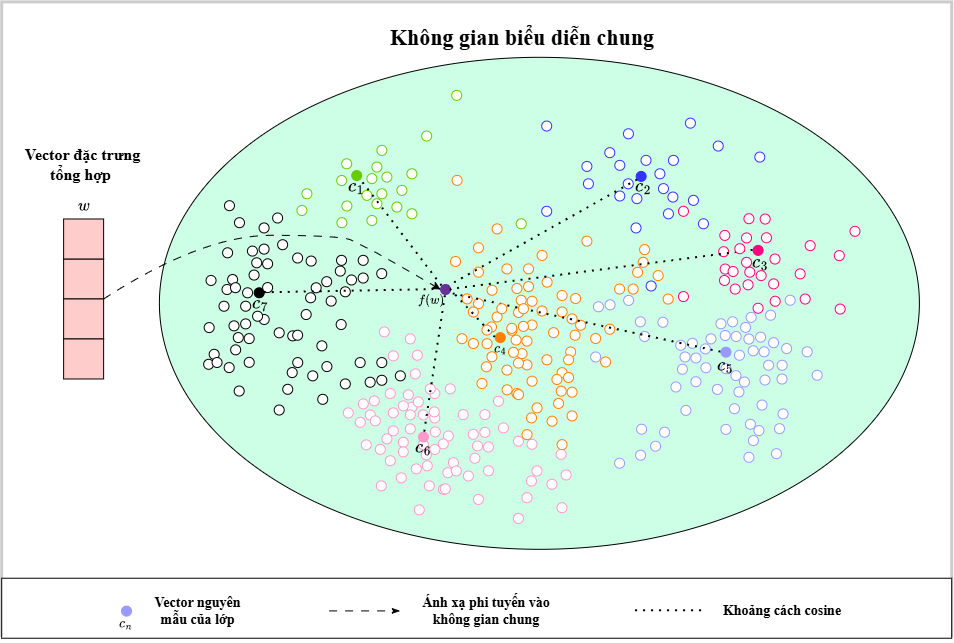
\includegraphics[width=0.92\textwidth]{images/protonet.png}
    \caption{Phân loại vectơ đặc trưng tổng hợp trong không gian nguyên mẫu}
    \label{fig:ch3_prototype}
\end{figure}

Với $\mathcal{I}_{k}=\left\{i\mid y_i=y_k\right\}$ là tập chỉ số các mẫu huấn luyện thuộc lớp $y_k$, nguyên mẫu lớp được ước lượng bằng trung bình đặc trưng:

\begin{equation}
\boldsymbol{c}_{k}
=
\frac{1}{\left|\mathcal{I}_{k}\right|}
\sum_{i\in\mathcal{I}_{k}}
\boldsymbol{z}_{i}.
\label{eq:ch3_prototype}
\end{equation}

Khoảng cách giữa mẫu mới và nguyên mẫu có thể được xây dựng từ độ tương đồng côsin:

\begin{equation}
d
\left(
\boldsymbol{z}_{i},
\boldsymbol{c}_{k}
\right)
=
1
-
\frac{
\boldsymbol{z}_{i}^{\mathsf{T}}\boldsymbol{c}_{k}
}{
\left\|\boldsymbol{z}_{i}\right\|_{2}
\left\|\boldsymbol{c}_{k}\right\|_{2}
}.
\label{eq:ch3_cosine_distance}
\end{equation}

Xác suất dự đoán được tính theo phân phối Softmax trên khoảng cách âm:

\begin{equation}
p
\left(
y_k\mid\boldsymbol{z}_{i}
\right)
=
\frac{
\exp
\left(
-d\left(\boldsymbol{z}_{i},\boldsymbol{c}_{k}\right)/\tau_c
\right)
}{
\sum_{j=1}^{K}
\exp
\left(
-d\left(\boldsymbol{z}_{i},\boldsymbol{c}_{j}\right)/\tau_c
\right)
},
\label{eq:ch3_prototype_probability}
\end{equation}

trong đó $\tau_c$ là hệ số nhiệt độ. Nhãn dự đoán là lớp có xác suất lớn nhất, tương đương với lớp có nguyên mẫu gần nhất theo độ đo đã chọn. Các nguyên mẫu là thống kê của tập huấn luyện, không phải tham số nhận đạo hàm. Khi biểu diễn thay đổi trong quá trình huấn luyện, các tâm lớp được ước lượng lại từ tập huấn luyện trước bước đánh giá.

\section{Huấn luyện hai giai đoạn trong quá trình ngoại tuyến}
\label{sec:ch3_offline_training}

\subsection{Giai đoạn 1: thích nghi miền bằng khớp ngữ nghĩa}
\label{subsec:ch3_phase1}

\begin{figure}[htbp]
    \centering
    
\includegraphics[width=0.84\textwidth]{images/domain.png}
    \caption{Giai đoạn thích nghi miền bằng khớp ngữ nghĩa ảnh-văn bản}
    \label{fig:ch3_phase1}
\end{figure}

Giai đoạn thứ nhất được minh họa trong Hình \ref{fig:ch3_phase1}. Ảnh X-quang và thông tin lâm sàng tương ứng được đưa qua hai bộ mã hóa để tạo các vectơ trong cùng một không gian. Các trọng số nền của BiomedCLIP được đóng băng, còn các ma trận LoRA và thành phần tổng hợp đặc trưng ảnh cục bộ được cập nhật. Mô-đun dung hợp và mạng nguyên mẫu chưa tham gia vào mục tiêu tối ưu ở giai đoạn này.

Giai đoạn này sử dụng hàm mất mát khớp ngữ nghĩa (Semantic Matching Loss) với phân phối đích mềm theo nhãn lớp. Trước hết, độ tương đồng giữa ảnh thứ $i$ và văn bản thứ $j$ được tính bằng độ tương đồng côsin có điều chỉnh nhiệt độ:

\begin{equation}
s_{ij}
=
\frac{
\overline{\boldsymbol{v}}_{i}^{\mathsf{T}}
\overline{\boldsymbol{t}}_{j}
}{
\tau_{\mathrm{SM}}
},
\label{eq:ch3_contrastive_similarity}
\end{equation}

trong đó $\overline{\boldsymbol{v}}_{i}$ và $\overline{\boldsymbol{t}}_{j}$ là các vectơ đã chuẩn hóa, còn $\tau_{\mathrm{SM}}$ là hệ số nhiệt độ. Biểu diễn ảnh dùng cho giai đoạn này lấy đặc trưng toàn cục làm điểm tựa và bổ sung tóm tắt có trọng số của các vùng cục bộ.

Với một lô gồm $B$ cặp ảnh-văn bản, trọng số đích mềm chưa chuẩn hóa được xác định theo quan hệ ngữ nghĩa giữa các cặp:

\begin{equation}
\widetilde{q}_{ij}
=
\mathbf{1}\left[i=j\right]
+
\rho\,
\mathbf{1}\left[i\neq j\right]
\mathbf{1}\left[y_i=y_j\right],
\qquad
0\leq\rho\leq 1.
\label{eq:ch3_semantic_target}
\end{equation}

Trong Công thức \ref{eq:ch3_semantic_target}, cặp ảnh-văn bản đúng của cùng một mẫu nhận trọng số lớn nhất, các cặp khác nhưng cùng nhãn nhận trọng số mềm $\rho$, còn các cặp khác lớp nhận trọng số bằng không. Các phân phối đích theo hai chiều được chuẩn hóa lần lượt theo hàng và theo cột:

\begin{equation}
\begin{aligned}
q_{ij}^{I\rightarrow T}
&=
\frac{\widetilde{q}_{ij}}
{\sum_{n=1}^{B}\widetilde{q}_{in}},
&
q_{ji}^{T\rightarrow I}
&=
\frac{\widetilde{q}_{ij}}
{\sum_{n=1}^{B}\widetilde{q}_{nj}}.
\end{aligned}
\label{eq:ch3_semantic_target_normalization}
\end{equation}

Từ các điểm tương đồng, mô hình tạo hai phân phối dự đoán:

\begin{equation}
\begin{aligned}
p_{ij}^{I\rightarrow T}
&=
\frac{\exp\left(s_{ij}\right)}
{\sum_{n=1}^{B}\exp\left(s_{in}\right)},
&
p_{ji}^{T\rightarrow I}
&=
\frac{\exp\left(s_{ij}\right)}
{\sum_{n=1}^{B}\exp\left(s_{nj}\right)}.
\end{aligned}
\label{eq:ch3_semantic_predictions}
\end{equation}

Hàm mất mát khớp ngữ nghĩa là trung bình của entropy chéo đích mềm theo hai chiều:

\begin{equation}
\mathcal{L}_{\mathrm{SM}}
=
-
\frac{1}{2B}
\sum_{i=1}^{B}
\sum_{j=1}^{B}
\left[
q_{ij}^{I\rightarrow T}
\log p_{ij}^{I\rightarrow T}
+
q_{ji}^{T\rightarrow I}
\log p_{ji}^{T\rightarrow I}
\right].
\label{eq:ch3_phase1_loss}
\end{equation}

Dạng mất mát trong Công thức \ref{eq:ch3_phase1_loss} kế thừa nguyên lý khớp ngữ nghĩa hai chiều của các mô hình ảnh-văn bản y khoa \cite{MedCLIP}. So với nhãn khớp cứng, phân phối đích mềm tránh xem mọi cặp khác mẫu là âm hoàn toàn khi chúng cùng mô tả một lớp bệnh. Việc lấy mẫu theo lớp làm tăng khả năng một lô có nhiều cặp cùng lớp để cung cấp tín hiệu ngữ nghĩa cho mục tiêu này.

\subsection{Giai đoạn 2: học dung hợp và phân loại}
\label{subsec:ch3_phase2}

\begin{figure}[htbp]
    \centering
    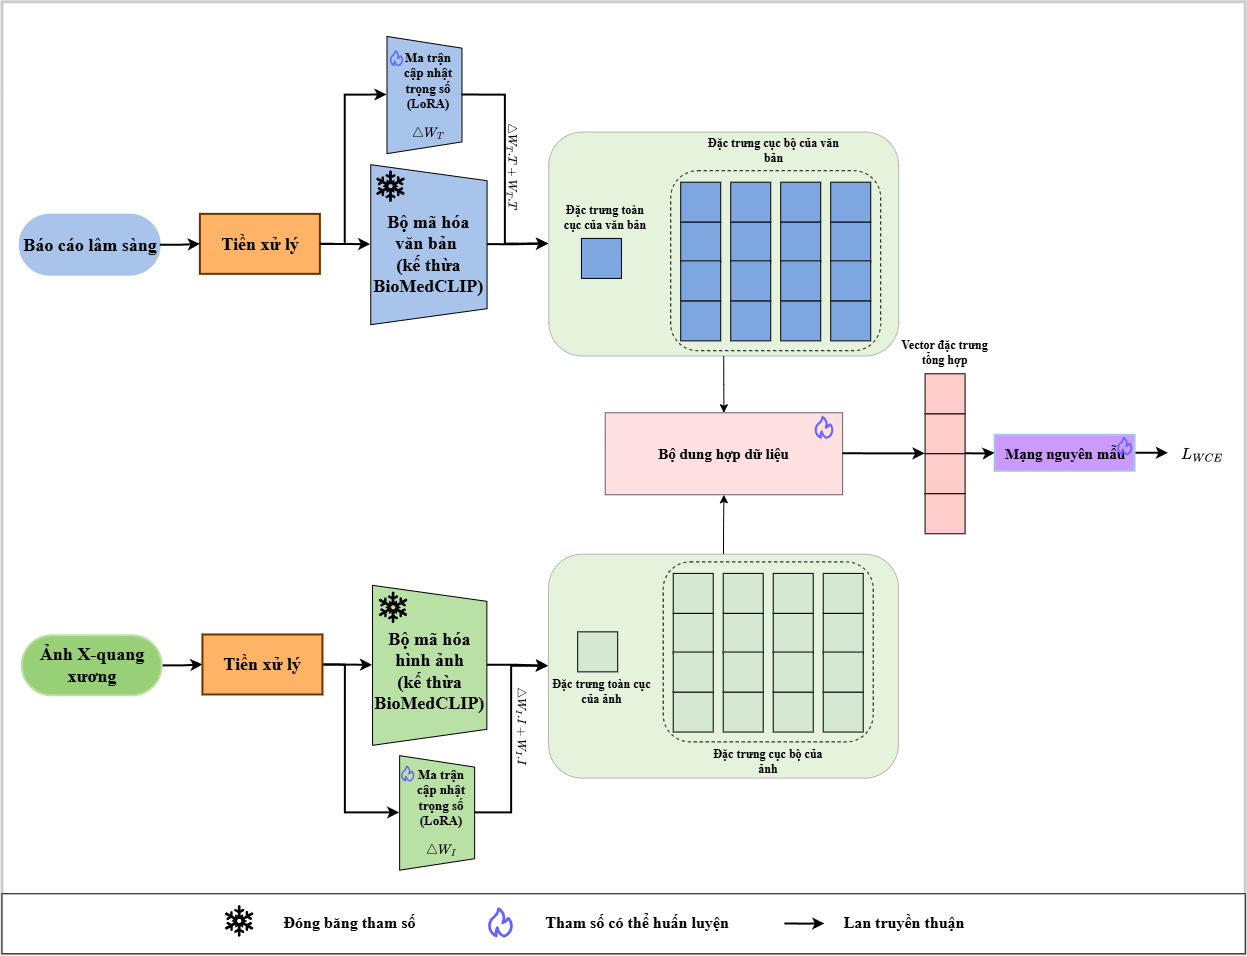
\includegraphics[width=0.90\textwidth]{images/classification.png}
    \caption{Giai đoạn học dung hợp và phân loại bằng mạng nguyên mẫu}
    \label{fig:ch3_phase2}
\end{figure}

Trong giai đoạn thứ hai, hai nhánh mã hóa tạo chuỗi đặc trưng toàn cục và cục bộ. Các chuỗi này được đưa qua mô-đun chú ý chéo để tạo vectơ tổng hợp $\boldsymbol{z}_{i}$. Mạng nguyên mẫu sử dụng các vectơ của tập huấn luyện để ước lượng tâm lớp và tính xác suất dự đoán. Trọng số nền của BiomedCLIP tiếp tục được giữ cố định, trong khi LoRA, thành phần biểu diễn ảnh cục bộ và mô-đun dung hợp được cập nhật.

Do số mẫu của các lớp có thể chênh lệch lớn, hàm mất mát sử dụng trọng số cân bằng lớp dựa trên số lượng mẫu hiệu dụng \cite{Cui2019ClassBalanced}. Với $n_k$ là số mẫu của lớp $k$, trọng số chưa chuẩn hóa được xác định bởi:

\begin{equation}
w_k
\propto
\frac{1-\beta}{1-\beta^{n_k}},
\qquad
0\leq\beta<1.
\label{eq:ch3_class_weight}
\end{equation}

Sau khi chuẩn hóa các trọng số để giữ thang đo ổn định, mục tiêu phân loại là entropy chéo có trọng số:

\begin{equation}
\mathcal{L}_{\mathrm{P2}}
=
-
\frac{1}{B}
\sum_{i=1}^{B}
w_{y_i}
\log
p
\left(
y=y_i
\mid
\boldsymbol{z}_{i}
\right).
\label{eq:ch3_phase2_loss}
\end{equation}

Sau mỗi chu kỳ huấn luyện, các nguyên mẫu được ước lượng lại bằng trạng thái hiện tại của mô hình trên tập huấn luyện, sau đó mới đánh giá trên tập kiểm định. Trạng thái mô hình tốt nhất được lựa chọn theo độ đo đã xác định trước trên tập kiểm định. Cuối cùng, các nguyên mẫu được tính lại từ tập huấn luyện bằng trạng thái đã chọn. Tập kiểm thử không được dùng để cập nhật tham số, ước lượng tâm lớp hoặc lựa chọn mô hình.

\section{Suy luận trong quá trình trực tuyến}
\label{sec:ch3_online_inference}

\begin{figure}[H]
    \centering
    
\includegraphics[width=\textwidth]{images/online.png}
    \caption{Quy trình suy luận trực tuyến và phát hiện mẫu ngoài phân phối}
    \label{fig:ch3_online}
\end{figure}

Khi tiếp nhận một ca mới, ảnh X-quang và thông tin lâm sàng được xử lý bằng đúng các phép biến đổi đã sử dụng trong huấn luyện. Hai bộ mã hóa tạo đặc trưng ảnh và văn bản, mô-đun chú ý chéo tạo vectơ tổng hợp, sau đó mạng nguyên mẫu tính xác suất cho từng lớp. Toàn bộ tham số LoRA, mô-đun dung hợp và các nguyên mẫu lớp đều được cố định. Quá trình này không tính đạo hàm và không cập nhật tâm lớp từ mẫu mới.

Ngoài kết quả phân loại, hệ thống hỗ trợ một mô-đun hậu xử lý tùy chọn để phát hiện mẫu ngoài phân phối. Một độ đo phổ biến là khoảng cách Mahalanobis từ biểu diễn tổng hợp đến lớp gần nhất \cite{Lee2018MahalanobisOOD}:

\begin{equation}
s_{\mathrm{OOD}}
\left(x^{img},x^{txt}\right)
=
\min_{k}
\left(
\boldsymbol{z}-\boldsymbol{\mu}_{k}
\right)^{\mathsf{T}}
\boldsymbol{\Sigma}^{-1}
\left(
\boldsymbol{z}-\boldsymbol{\mu}_{k}
\right),
\label{eq:ch3_ood_score}
\end{equation}

trong đó $\boldsymbol{\mu}_{k}$ là tâm đặc trưng của lớp $k$ và $\boldsymbol{\Sigma}$ là ma trận hiệp phương sai được ước lượng từ dữ liệu trong phân phối, còn $\boldsymbol{z}$ là biểu diễn tổng hợp của $x^{img}$ và $x^{txt}$. Ngưỡng $\tau$ được hiệu chỉnh chỉ bằng dữ liệu huấn luyện và kiểm định. Thống nhất với ký hiệu ở Chương 1, quy tắc đầu ra của hệ thống là:

\begin{equation}
\widehat{y}
=
\begin{cases}
\mathrm{OOD},
& \text{nếu }s_{\mathrm{OOD}}\left(x^{img},x^{txt}\right)>\tau,\\[4pt]
\displaystyle
\operatorname*{arg\,max}_{y_k\in\mathcal{Y}}
p\left(y_k\mid x^{img},x^{txt}\right),
& \text{ngược lại}.
\end{cases}
\label{eq:ch3_ood_decision}
\end{equation}

Mô-đun phát hiện ngoài phân phối không thay đổi dự đoán nội tại của XBone-Net. Nó cung cấp thêm một tín hiệu cảnh báo về mức độ phù hợp của mẫu với phân bố đã quan sát. Vì vậy, đầu ra phân loại và cảnh báo ngoài phân phối có hai vai trò khác nhau: đầu ra thứ nhất chọn lớp gần nhất trong tập lớp đã biết, còn đầu ra thứ hai đánh giá liệu quyết định đó có được thực hiện trên một mẫu đủ quen thuộc hay không.

\section{Tóm tắt chương}

Chương này đã trình bày XBone-Net theo luồng từ tổng quan đến từng thành phần. Nhánh ảnh sử dụng bộ mã hóa thị giác kế thừa từ BiomedCLIP và cơ chế xử lý độ phân giải cao để kết hợp bối cảnh toàn cục với chi tiết cục bộ. Nhánh văn bản mã hóa thông tin lâm sàng trong cùng không gian đặc trưng. LoRA thích nghi hai bộ mã hóa với số tham số huấn luyện nhỏ, cơ chế chú ý chéo hai chiều trao đổi thông tin giữa hai phương thức và mạng nguyên mẫu thực hiện quyết định theo khoảng cách đến tâm lớp.

Quy trình huấn luyện gồm hai giai đoạn ngoại tuyến. Giai đoạn thứ nhất căn chỉnh biểu diễn ảnh-văn bản bằng hàm mất mát khớp ngữ nghĩa, còn giai đoạn thứ hai tối ưu biểu diễn dung hợp và mục tiêu phân loại có cân bằng lớp. Trong quá trình trực tuyến, mô hình giữ cố định toàn bộ tham số, thực hiện phân loại cho ca mới và có thể bổ sung cảnh báo ngoài phân phối đã được hiệu chỉnh trước.
